\def\duedate{10/27/22}
\def\HWnum{2}
% Document setup
\documentclass[12pt]{article}
\usepackage[margin=1in]{geometry}
\usepackage{fancyhdr}
\usepackage{lastpage}

\pagestyle{fancy}
\lhead{Richard Whitehill}
\chead{PHYS 714 -- HW \HWnum}
\rhead{\duedate}
\cfoot{\thepage \hspace{1pt} of \pageref{LastPage}}

% Encoding
\usepackage[utf8]{inputenc}
\usepackage[T1]{fontenc}

% Math/Physics Packages
\usepackage{amsmath}
\usepackage{amssymb}
\usepackage{dsfont}
\usepackage{mathtools}
\usepackage[arrowdel]{physics}
\usepackage{siunitx}

\AtBeginDocument{\RenewCommandCopy\qty\SI}

% Reference Style
\usepackage{hyperref}
\hypersetup{
    colorlinks=true,
    linkcolor=blue,
    filecolor=magenta,
    urlcolor=cyan,
    citecolor=green
}

\newcommand{\eref}[1]{Eq.~(\ref{eq:#1})}
\newcommand{\erefs}[2]{Eqs.~(\ref{eq:#1})--(\ref{eq:#2})}

\newcommand{\fref}[1]{Fig.~\ref{fig:#1}}
\newcommand{\frefs}[2]{Figs.~\ref{fig:#1}--\ref{fig:#2}}

\newcommand{\tref}[1]{Table~\ref{tab:#1}}
\newcommand{\trefs}[2]{Tables~\ref{tab:#1}-\ref{tab:#2}}

% Figures and Tables 
\usepackage{graphicx}
\usepackage{float}

\newcommand{\bef}{\begin{figure}[h!]\begin{center}}
\newcommand{\eef}{\end{center}\end{figure}}

\newcommand{\bet}{\begin{table}[h!]\begin{center}}
\newcommand{\eet}{\end{center}\end{table}}

% tikz
\usepackage{tikz}
\usetikzlibrary{calc}
\usetikzlibrary{decorations.pathmorphing}
\usetikzlibrary{decorations.markings}
\usetikzlibrary{arrows.meta}
\usetikzlibrary{positioning}

% tcolorbox
\usepackage[most]{tcolorbox}
\usepackage{xcolor}
\usepackage{xifthen}
\usepackage{parskip}

\newcommand*{\eqbox}{\tcboxmath[
    enhanced,
    colback=black!10!white,
    colframe=black,
    sharp corners,
    size=fbox,
    boxsep=8pt,
    boxrule=1pt
]}

% Miscellaneous Definitions/Settings
\newcommand{\prob}[2]{\textbf{#1)} #2}

\setlength{\parskip}{\baselineskip}
\setlength{\parindent}{0pt}

\def\complexs{\mathbb{C}}
\def\reals{\mathbb{R}}
\def\naturals{\mathbb{N}}
\def\integers{\mathbb{Z}}
\def\rationals{\mathbb{Q}}
\def\id{\mathds{1}}



\begin{document}
    
\prob{1}{
Find the $LU$, $LDU$, and $LDL^{\rm T}$ factorization of the matrix
\begin{eqnarray}
    \label{eq:mat-A}
    A = 
    \begin{pmatrix}
        1 & -1 & 2 & 0 \\
        -1 & 2 & -3 & 1 \\
        2 & -3 & 1 & 3 \\
        0 & 1 & 3 & -4
    \end{pmatrix}
.\end{eqnarray}
}

We can find the $LU$ factorization by performing Gaussian elimination, recording the coefficients to find the $L$ matrix, and the remaining upper triangular matrix is $U$:
\begin{align}
    \label{eq:A-Gaussian}
    A = 
    \begin{pmatrix}
        1 & -1 & 2 & 0 \\
        -1 & 2 & -3 & 1 \\
        2 & -3 & 1 & 3 \\
        0 & 1 & 3 & -4
    \end{pmatrix}
    &\stackrel{1}{\rightarrow}
    \begin{pmatrix}
        1 & -1 & 2 & 0 \\
        0 & 1 & -1 & 1 \\
        0 & -1 & -3 & 3 \\
        0 & 1 & 3 & -4
    \end{pmatrix}
    \stackrel{2}{\rightarrow}
    \begin{pmatrix}
        1 & -1 & 2 & 0 \\
        0 & 1 & -1 & 1 \\
        0 & 0 & -4 & 4 \\
        0 & 0 & 4 & -5
    \end{pmatrix} \\
    &\stackrel{3}{\rightarrow}
    \eqbox{
    \begin{pmatrix}
        1 & -1 & 2 & 0 \\
        0 & 1 & -1 & 1 \\
        0 & 0 & -4 & 4 \\
        0 & 0 & 0 & -1
    \end{pmatrix} 
    = U}
,\end{align}
where
\begin{eqnarray}
    \label{eq:L-mats}
    \tilde{L}_1 = 
    \begin{pmatrix}
        1 & 0 & 0 & 0 \\
        1 & 1 & 0 & 0 \\
        -2 & 0 & 1 & 0 \\
        0 & 0 & 0 & 1
    \end{pmatrix}
    \quad
    \tilde{L}_{2} = 
    \begin{pmatrix}
        1 & 0 & 0 & 0 \\
        0 & 1 & 0 & 0 \\
        0 & 1 & 1 & 0 \\
        0 & -1 & 0 & 1 
    \end{pmatrix}
    \quad
    \tilde{L}_{3} = 
    \begin{pmatrix}
        1 & 0 & 0 & 0 \\
        0 & 1 & 0 & 0 \\
        0 & 0 & 1 & 0 \\
        0 & 0 & 1 & 1 
    \end{pmatrix}
,\end{eqnarray}
meaning
\begin{align}
    \label{eq:L-from-123}
    L &= (\tilde{L}_{3}\tilde{L}_{2}\tilde{L}_{1})^{-1} = \tilde{L}_{1}^{-1} \tilde{L}_{2}^{-1} \tilde{L}_{3}^{-1} \\
    &=
    \begin{pmatrix}
        1 & 0 & 0 & 0 \\
        -1 & 1 & 0 & 0 \\
        2 & 0 & 1 & 0 \\
        0 & 0 & 0 & 1 
    \end{pmatrix}
    \begin{pmatrix}
        1 & 0 & 0 & 0 \\
        0 & 1 & 0 & 0 \\
        0 & -1 & 1 & 0 \\
        0 & 1 & 0 & 1 
    \end{pmatrix}
    \begin{pmatrix}
        1 & 0 & 0 & 0 \\
        0 & 1 & 0 & 0 \\
        0 & 0 & 1 & 0 \\
        0 & 0 & -1 & 1
    \end{pmatrix} \\
    &= 
    \eqbox{
    \begin{pmatrix}
        1 & 0 & 0 & 0 \\
        -1 & 1 & 0 & 0 \\
        2 & -1 & 1 & 0 \\
        0 & 1 & -1 & 1
    \end{pmatrix}
}
.\end{align}
We can write the $LDU$ factorization by letting
\begin{eqnarray}
    \label{eq:D-mat}
    \eqbox{
    D = 
    \begin{pmatrix}
        1 & 0 & 0 & 0 \\
        0 & 1 & 0 & 0 \\
        0 & 0 & -4 & 0 \\
        0 & 0 & 0 & -1
    \end{pmatrix}
}
,\end{eqnarray}
which makes
\begin{eqnarray}
    \label{eq:U-D}
    \eqbox{
    U =
    \begin{pmatrix}
        1 & -1 & 2 & 0 \\
        0 & -1 & 1 & 0 \\
        0 & 0 & 1 & -1 \\
        0 & 0 & 0 & 1
    \end{pmatrix}
    = L^{\rm T}
}
,\end{eqnarray}
which also conveniently gives us our $LDL^{\rm T}$ factorization of $A$.


\prob{2}{
Let $A$ be an upper triangular $n \times n$ matrix and $b$ be an $n$-vector.
}

a) Please write out the algorithm to solve $Ax = b$ by backward substitution, and calculate flops.

The algorithm is as follows:
\begin{verbatim}
    x(n) = b(n)/A(n,n) 
    For i = n-1:1:-1
        x(i) = (y(i) - sum([x(k)*A(i,k) for k=i+1:n]))/A(i,i)
    end
\end{verbatim}
The flops can be calculated as follows (ignoring assignment operations).
At the $i^{\rm th}$ step (for $i = 1, 2, \ldots, n$) we have 1 multiplication, 1 subtraction, $n-i$ multiplications, and $n-i-1$ additions.
Thus,
\begin{align}
    \label{eq:flops-backward}
    \eqbox{
    \begin{aligned}
    {\rm flops} &= \sum_{i=1}^{n} [1 + 1 + (n-i) + (n-i-1)] = \sum_{i=1}^{n} [2n + 1 - 2i] \\
                &= n(2n+1) - n(n+1) = n^2 = \mathcal{O}(n^2)
    \end{aligned}
}
.\end{align}


b) Perform round-off error analysis, i.e. the substitution algorithm is backward stable in the sense that $(A + \delta A) \hat{x} = b$ with
\begin{eqnarray}
    \label{eq:error}
    \frac{|\delta a_{ij}|}{|a_{ij}|} \leq n \epsilon + \mathcal{O}(\epsilon^2)
,\end{eqnarray}
where $\epsilon$ is the machine precision, $\delta a_{ij}$  is the $(i,j)$-entry in $\delta A$, and $a_{ij}$ is the $(i,j)$-entry in $A$.

We would like to show the equivalent result
\begin{eqnarray}
    \label{eq:res-b}
    | \delta A | \leq n\epsilon | A | + \mathcal{O}(\epsilon^2)
.\end{eqnarray}
Note that we can write $Ax = b$ in expanded form as
\begin{eqnarray}
    \label{eq:expand-Axb}
    \begin{cases}
        a_{11} x_1 + a_{12} x_2 + \ldots + a_{1n} x_{n} &= b_{1} \\
        \phantom{a_{11} x_1 +} a_{22} x_2 + \ldots + a_{2n} x_{n} &= b_{2} \\
        \phantom{a_{11} x_1 + a_{22} x_2 + \ldots + a_{2n} x_{n}} &\vdots \\
        \phantom{a_{11} x_1 + a_{22} x_2 + \ldots + } a_{nn} x_{n} &= b_{n} \\
    \end{cases} 
.\end{eqnarray}
This is solved using back-substitution:
\begin{align}
    \label{eq:back-sub}
    x_{n} &= b_{n}/a_{nn} \\
    x_{j} &= \frac{b_{i} - \sum_{k=j-1}^{n} a_{jk} x_{k}}{a_{ii}}
.\end{align}
To analyze the error we can use floating point arithmetic, making note that this is a recursive process (i.e. each successive calculation depends on the floating point errors accumulated in the previous caluculations).
Consider the following algorithm:
\begin{verbatim}
w(1) = b(i) 
For j = n,n-1,...,i-1
    w(j+1) = w(j) - a(i,j)x(j)
end
x(i) = w(i)/a(i,i)
\end{verbatim}
Then,
\begin{align}
    \label{eq:float-calc}
    {\rm fl}(w^{(j+1)}) &= ({\rm fl}(w^{(j)}) - a_{ij}x_{j}(1 + \delta_{j}))(1 + \delta_{j}') \\
    x_{i} a_{ii} &= (1 + \delta_{i}) {\rm fl}(w^{i})
\end{align}
for $j = n,n-1,\ldots,i-1$.
Expanding \eref{float-calc} explicitly, then
\begin{gather}
    \label{eq:float-calc-expand}
    \frac{a_{ii}x_{i}}{1 + \delta_{i}} = b_{i}(1 + \delta_{n}')(1 + \delta_{n-1}')\hdots(1+\delta_{i-1}') - \sum_{j=i-1}^{n} a_{ij} x_{j} (1 + \delta_{j})(1+\delta_{n}')\hdots(1+\delta_{i-1}') \\
    \frac{a_{ii}x_{i}}{(1 + \delta_{i})(1+\delta_{n}')\hdots(1+\delta_{i-1}')} = b_{i} - \sum_{j=i-1}^{n} a_{ij} x_{j} \frac{(1 + \delta_{j}}{(1+\delta_{n}')\hdots(1+\delta_{j-1}')}
.\end{gather}
Thus, 
\begin{eqnarray}
    \label{eq:redefine-last}
    \tilde{a}_{ii} x_{i} = b_{i} - \sum_{j=i-1}^{n} \tilde{a}_{ij} x_{j}
,\end{eqnarray}
where
\begin{eqnarray}
    \label{eq:define-tilde-a}
    \tilde{a}_{ii} = \frac{a_{ii}}{(1+\delta_{i})(1+\delta_{n}')\ldots(1+\delta_{i-1}')} = (1 + \epsilon_{ii}) a_{ii}
.\end{eqnarray}
Furthermore,
\begin{eqnarray}
    \label{eq:define-tilde-a-1}
    \tilde{a}_{ij} = \frac{(1+\delta_{j}) a_{ij}}{(1+\delta_{n}')\ldots(1+\delta_{j-1}')} = a_{ij}(1+\epsilon_{ij})
.\end{eqnarray}
Observe that
\begin{eqnarray}
    \label{eq:epsilon-def}
    \epsilon_{jj} \leq j \epsilon + \mathcal{O}(\epsilon^2) \leq n \epsilon + \mathcal{O}(\epsilon^2)
,\end{eqnarray}
for some $\epsilon \in \reals$.
That is,
\begin{eqnarray}
    \label{eq:float-point-eq}
    (A + \delta A) \hat{x} = b
,\end{eqnarray}
where
\begin{eqnarray}
    \label{eq:delta-A}
    |\delta A| \leq n\epsilon |\delta A| + \mathcal{O}(\epsilon^2)
.\end{eqnarray}



\prob{3}{
Let $A,\delta A \in \reals^{n \times n}$ be full rank and $b,x,\delta x \in \reals^{n}$.
Prove that if $Ax = b$ and $(A + \delta A)(x + \delta x) = b$, then
\begin{eqnarray}
    \label{eq:errors-3}
    \frac{|| \delta x ||}{|| x + \delta x ||} \leq \kappa(A) \frac{|| \delta A ||}{ || A ||}
,\end{eqnarray}
where $\kappa(A)$ is the condition number of $A$ and $|| \cdot ||$ is any norm.
}

The second equality gives us
\begin{align}
    \label{eq:expand-2}
    (A + \delta A)(x + \delta x) &= Ax + A \delta x + \delta A (x + \delta x) = b \\
    A \delta x + \delta A (x + \delta x) &= 0
.\end{align}
Rearranging and multiplying both sides by $A^{-1}$, which exists since $A x = b$ has unique solution for nontrivial $b$, we find
\begin{gather}
    \label{eq:delta-x}
    \delta x = - A^{-1} \delta A (x + \delta x) \Rightarrow || \delta x || = || A^{-1} \delta A (x + \delta x) || \leq || A^{-1} ||\,|| \delta A ||\,|| x + \delta x || \\
    \eqbox{
    \frac{|| \delta x ||}{|| x + \delta x ||} \leq || A^{-1} ||\,|| \delta A || = \kappa(A) \frac{|| \delta A ||}{|| A ||}
}
.\end{gather}


\prob{4}{
Solve the following linear system by direct method via hand calculation and computer programming:
\begin{eqnarray}
    \label{eq:system}
    \begin{cases}
    4 x_1 + x_2 - x_3 + x_4 = -2 \\
    x_1 + 4x_2 - x_3 - x_4 = -1 \\
    -x_1 - x_2 + 5x_3 + x_4 = 0 \\
    x_1 - x_2 + x_3 + 3x_4 = 1
    \end{cases} 
.\end{eqnarray}
}

The system above is equivalent to the matrix equation $Ax = b$, which can be solved using Gaussian elimination via the following ``augmented'' matrix:
\begin{align}
    \label{eq:A-b}
    \begin{pmatrix}
        4 & 1 & -1 & 1 & -2 \\
        1 & 4 & -1 & -1 & -1 \\
        -1 & -1 & 5 & 1 & 0 \\
        1 & -1 & 1 & 3 & 1
    \end{pmatrix}
    &\rightarrow
    \begin{pmatrix}
        1 & 1/4 & -1/4 & 1/4 & -1/2 \\
        1 & 4 & -1 & -1 & -1 \\
        -1 & -1 & 5 & 1 & 0 \\
        1 & -1 & 1 & 3 & 1
    \end{pmatrix}
    \\
    &\rightarrow
    \begin{pmatrix}
        1 & 1/4 & -1/4 & 1/4 & -1/2 \\
        0 & 15/4 & -3/4 & -5/4 & -1/2 \\
        0 & -3/4 & 19/4 & 5/4 & -1/2 \\
        0 & -5/4 & 5/4 & 11/4 & 3/2
    \end{pmatrix}
    \\
    &\rightarrow
    \begin{pmatrix}
        1 & 1/4 & -1/4 & 1/4 & -1/2 \\
        0 & 1 & -1/5 & -1/3 & -2/15 \\
        0 & -3/4 & 19/4 & 5/4 & -1/2 \\
        0 & -5/4 & 5/4 & 11/4 & 3/2
    \end{pmatrix}
    \\
    &\rightarrow
    \begin{pmatrix}
        1 & 0 & -1/5 & 1/3 & -7/15 \\
        0 & 1 & -1/5 & -1/3 & -2/15 \\
        0 & 0 & 23/5 & 1 & -3/5 \\
        0 & 0 & 1 & 7/3 & 4/3
    \end{pmatrix}
    \\
    &\rightarrow
    \begin{pmatrix}
        1 & 0 & -1/5 & 1/3 & -7/15 \\
        0 & 1 & -1/5 & -1/3 & -2/15 \\
        0 & 0 & 1 & 5/23 & -3/23 \\
        0 & 0 & 1 & 7/3 & 4/3
    \end{pmatrix}
    \\
    &\rightarrow
    \begin{pmatrix}
        1 & 0 & -1/5 & 1/3 & -34/69 \\
        0 & 1 & -1/5 & -1/3 & 11/69 \\
        0 & 0 & 1 & 5/23 & -3/23 \\
        0 & 0 & 0 & 146/69 & 101/69
    \end{pmatrix}
    \\
    &\rightarrow
    \begin{pmatrix}
        1 & 0 & 0 & 26/69 & -34/69 \\
        0 & 1 & 0 & -20/69 & 11/69 \\
        0 & 0 & 1 & 5/23 & -3/23 \\
        0 & 0 & 0 & 146/69 & 101/69
    \end{pmatrix}
    \\
    &\rightarrow
    \begin{pmatrix}
        1 & 0 & 0 & 0 & -55/73 \\
        0 & 1 & 0 & 0 & 3/73 \\
        0 & 0 & 1 & 0 & -41/146 \\
        0 & 0 & 0 & 1 & 101/146 
    \end{pmatrix}
.\end{align}
Thus, 
\begin{eqnarray}
    \label{eq:x-sol}
    x = 
    \begin{pmatrix}
        -55/73 & 3/73 & -41/146 & 101/146    
    \end{pmatrix}^{\rm T}
.\end{eqnarray}

This problem was solved numerically using the program below.

\newpage
\inputpython{prob4.py}

The solution is shown in the image below: 
\begin{center}
    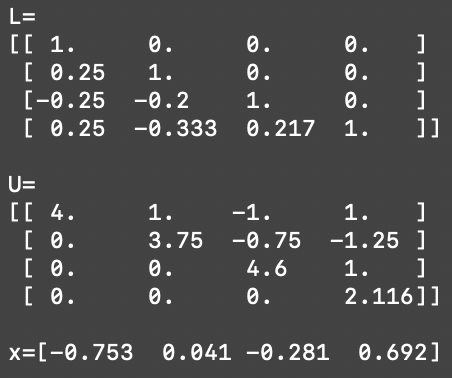
\includegraphics[width=0.6\textwidth]{prob4_comp.png}
\end{center}

\prob{5}{
Show how $LU$ factorization with partial pivoting works for the matrix via hand calculation and computer programming:
\begin{eqnarray}
    \label{eq:A-pivoting}
    A = 
    \begin{pmatrix}
        4 & 7 & 3 \\
        1 & 3 & 2 \\
        2 & -4 & -1
    \end{pmatrix}
.\end{eqnarray}
Give the $P$, $L$, and $U$ matrices.
}

The $LU$ factorization with partial pivoting for this matrix occurs as follows:
\begin{align}
    \label{eq:PLU-factorization}
    \begin{pmatrix}
        4 & 7 & 3 \\
        1 & 3 & 2 \\
        2 & -4 & -1
    \end{pmatrix}
    &\stackrel{1}{\rightarrow}
    \begin{pmatrix}
        4 & 7 & 3 \\
        0 & 5/4 & 5/4 \\
        0 & -15/2 & -5/2
    \end{pmatrix}
    \stackrel{2}{\rightarrow}
    \begin{pmatrix}
        4 & 7 & 3 \\
        0 & -15/2 & -5/2 \\
        0 & 5/4 & 5/4
    \end{pmatrix} 
    \\
    &\stackrel{3}{\rightarrow}
    \begin{pmatrix}
        4 & 7 & 3 \\
        0 & -15/2 & -5/2 \\
        0 & 0 & 5/6 \\
    \end{pmatrix}
    = U
.\end{align}
Thus, 
\begin{eqnarray}
    \label{eq:P-mat}
    P = 
    \begin{pmatrix}
        1 & 0 & 0 \\
        0 & 0 & 1 \\
        0 & 1 & 0
    \end{pmatrix}
,\end{eqnarray}
and 
\begin{eqnarray}
    \label{eq:Lmats}
    L_{1} = 
    \begin{pmatrix}
        1 & 0 & 0 \\
        -1/4 & 1 & 0 \\
        -1/2 & 0 & 1 
    \end{pmatrix}
    ~
    L_{2} = 
    \begin{pmatrix}
        1 & 0 & 0 \\
        0 & 1 & 0 \\
        0 & -1/6 & 0
    \end{pmatrix}
    \Rightarrow
    L = P L_1 P L_2 = 
    \begin{pmatrix}
        1 & 0 & 0 \\
        -1/2 & 1 & 0 \\
        -1/4 & -1/6 & 1
    \end{pmatrix}
.\end{eqnarray}

The program below shows the algorithm to factor a matrix as $A = PLU$:

\inputpython{prob5.py}

The output of the code above is displayed in the image below:

\begin{center}
    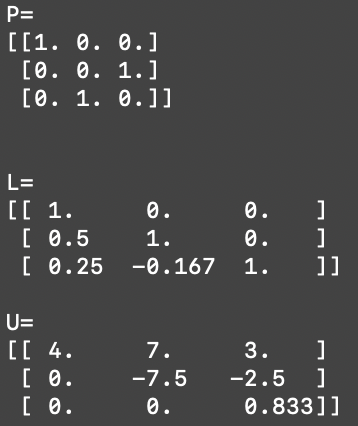
\includegraphics{prob5.png} 
\end{center}


\end{document}
